\chapter{Detailed Problem Requirements}
\section{Target Environment}

The goal of the head-tracking system was to determine the position and orientation in the specific target environment of KU Leuven's Group T Campus's spiral walkway. During the course of our research, we received the ground plans for the building.

\begin{figure}[h] 
	\centering 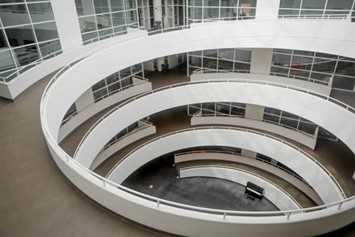
\includegraphics[height=5cm]{./images/spiral_groupt.jpg}
	\caption{The target environment for this project, Campus GroupT's spiral walkway (Leuven, Belgium).}
\end{figure}

\section{Sensors and MCUs}

Our project used the Bosch BNO055, a 9-axis intelligent absolute orientation sensor, and the BMP390, a high-precision barometric pressure sensor, for motion and altitude tracking, respectively. The BNO055 integrates a gyroscope, accelerometer, and magnetometer with an onboard microcontroller that fuses sensor data, offering orientation accuracy of  \textpm 1\textdegree \ in stable conditions.  \cite{bno055} Its self-calibrating features reduced the complexity of manual calibration, though environmental interference occasionally introduced noise. The BMP390 ensured altitude measurements in the precision of \textpm 0.03 hPa, thereby allowing for height estimations within a range of \textpm 0.25 meters. \cite{bmp390}

\begin{figure}[h] 
	\centering 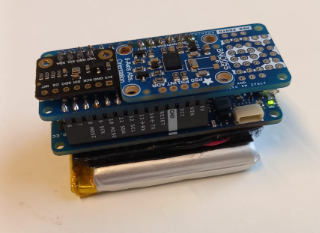
\includegraphics[height=5cm]{./images/hamburger.png}
	\caption{The Arduino module and sensors used.}
\end{figure}